\documentclass{article}
\usepackage[utf8]{inputenc}
\usepackage{amsmath}
\usepackage{graphicx}
\usepackage{multirow}
\usepackage{biblatex}
\usepackage{multicol}
\usepackage{subcaption}
\usepackage{authblk}
\usepackage{todonotes}

\title{ SimAN: Exploring Self-Supervised Representation Learning of Scene Text
via Similarity-Aware Normalization}
\vspace{20pt}

\author[1]{\raggedright Canjie Luo}
\author[1,2,$\asteric$]{\raggedright Lianwen Jin}
\author[3]{\raggedright Jingdong Chen}


\affil[1]{South China University of Technology, }
\affil[2]{Peng Cheng Laboratory,} 
\affil[3]{Ant Group}
\footnotesize \verb|\{canjie.luo, lianwen.jin\verb|\}@gmail.com, jingdongchen.cjd@antgroup.com
\newline

\addbibresource{biblio.bib}
\begin{document}

\maketitle

\begin{multicols}{2}
\begin{abstract}
    Recently self-supervised representation learning has
drawn considerable attention from the scene text recognition
community. Different from previous studies using contrastive
learning, we tackle the issue from an alternative
perspective, i.e., by formulating the representation learning
scheme in a generative manner. Typically, the neighboring
image patches among one text line tend to have similar
styles, including the strokes, textures, colors, etc. Motivated
by this common sense, we augment one image patch
and use its neighboring patch as guidance to recover itself.
Specifically, we propose a Similarity-Aware Normalization
(SimAN) module to identify the different patterns and align
the corresponding styles from the guiding patch. In this
way, the network gains representation capability for distinguishing
complex patterns such as messy strokes and cluttered
backgrounds. Experiments show that the proposed
SimAN significantly improves the representation quality and
achieves promising performance. Moreover, we surprisingly
find that our self-supervised generative network has
impressive potential for data synthesis, text image editing,
and font interpolation, which suggests that the proposed
SimAN has a wide range of practical applications.

\end{abstract}

\section{Introduction}
To summarize, our contributions are as follows:
\begin{itemize}
    \item We propose a generative (opposite of contrastive [34])
representation learning scheme by utilizing the unique
properties of scene text, which might inspire rethinking
the learning of better representations for sequential
data like text images. To the best of our knowledge,
this is the first attempt for scene text recognition.

    \item We propose a SimAN module, which estimates the
similarity of the representations between the aug augmented
image patch and its neighboring patch to align
corresponding styles. Only if the representations are
sufficiently distinguishable, different patterns can be
identified and be aligned with correct styles. Otherwise,
the network might result in a wrong recovered
image, e.g., in different colors.

    \item The proposed SimAN achieves promising representation
performance. Moreover, the self-supervised network
shows impressive capabilities to synthesize data,
edit text images and interpolate fonts, suggesting the
broad practical applications of the proposed approach.
\end{itemize}

\section{Related Work}



\section{Methodology}
In this section, we first introduce the design of the pretext
task and the construction of the training samples. Then, we
detail the proposed SimAN module. Finally, we present the
objectives of the task and the complete learning scheme.
The overall framework is shown in Figure 2.

\subsection{Training Sample Construction}
Constructing appropriate training samples is critical to
the success of the pretext task. We enable the scene text
representation learning by recovering an augmented image
patch using its neighboring patch as guidance. This design
considers the unique properties of scene text, i.e., the styles
(e.g., stroke width, textures, and colors) within one text line
tend to be consistent.
The pretext task requires decoupled style and content inputs.
As shown in Figure 2, given an unlabeled text image
$I ∈ R^{3×H×W}$ (the width W is required to be larger than
two times of height H), we randomly crop two neighboring
image patches $I_s, I_c ∈ R^{3×H×H} $as style and content
input, respectively. This ensures sufficient differences in
content between the two patches. Even if the neighboring
patches might contain a same characters, their positions are
different. Then, we augment (blurring, random noise, color
changes, etc.) the content patch $I_c$ as $I_aug$ to make its style different from the style patch $I_s$. Finally, the pretext task
takes $I_aug$ as content input and $I_s$ as the style guidance to
recover an image $I_rec$. The source content patch $I_c$ serves
as supervision. \\

\textbf{Discussion} As our pretext task is recovering an augmented patch under the guidance of its neighboring patch,
the visual cues should be consistent in both patches. Some
spatial augmentation strategies, such as elastic transformation,
might break the consistency and lead to failed training.
For instance, it might bring changes to the stroke width.
The excessively distorted strokes are also diverse from the
source font style. Therefore, we avoid all of the spatial
transformation augmentation methods that are widely used
for self-supervised representation learning. This is also a
significant difference with previous study SeqCLR [1].

\subsubsection{Similarity-Aware Normalization}
\ref{eq1}
\begin{equation}
    \mathcal{\sigma}_{c,i,j} = \frac{1}{3}{\sqrt{\sum_{p,q N_{i,j}} (x_{c,p,q} - \mu_{c,i,j})^2 } }
    \label{eq1}
\end{equation}
\end{multicols}

\subsection{Learning Scheme}

\begin{table}[ht]
    \centering
    \begin{tabular}{c}
    \hline
        \textbf{Algorithm 1} Representation Learning Scheme\\
        \hline
        \textbf{Output:} Encoder, Decoder\\
1: for iteration t = 0, 1, 2, \cdots, T do \\
2: Sample a mini-batch {Ii}B\\
i=1 from unlabeled data
3: for each $I_i$ do\\
4: Randomly crop $I_s$ and $I_c$, augment $I_c$ as $I_aug$\\
5: Forward Encoder, SimAN and Decoder\\
6: Compute loss for {Irec,i}B
i=1||
7: Update D using minDLadv\\
8: Update Encoder and Decoder using
min
Encoder, Decoder
Ladv + λL2\\
9: (The λ is empirically set to 10.)\\
\hline
    \end{tabular}
    \caption{algo}
    \label{tab:algo}
\end{table}

\section{}
\subsection{}
\subsection{Implementation Details}
architectures,
probe objectives, and training settings, in the Supplementary
Material.
Encoder/Decoder We adopt a popular recognizer backbone
ResNet-29 [2] as our encoder. We symmetrically design
a lightweight decoder.
Recognizer The complete architecture of the recognizer
follows [1,2], including a rectification module, a ResNet-29
backbone, two stacked BiLSTMs and a CTC [15] /Attention
[4] decoder, as shown in Figure 3.
Optimization In the self-supervised representation
learning stage, we set the batch size to 256 and train the
network for 400K iterations. It takes less than 3 days for
convergence on two NVIDIA P100 GPUs (16GB memory
per GPU). The optimizer is Adam [30] with the settings
of β1 = 0.5 and β2 = 0.999. The learning rate is set to
10−4 and linearly decreased to 10−5. The images are resized
to a height of 32 pixels, maintaining the aspect ratio.
The training setting of recognizers follows previous study
SeqCLR [1].


\section{Acknowledgment}
This research was supported in part by NSFC (Grant No.
61936003) and GD-NSF (No. 2017A030312006).

\begin{figure}
    \centering
    \begin{subfigure}[b]{0.3\textwidth}
        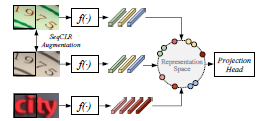
\includegraphics[width=\textwidth]{figure1.png}
        \caption{Contrastive representation learning}
        \label{fig:gull}
    \end{subfigure}
    
    \begin{subfigure}[b]{0.3\textwidth}
        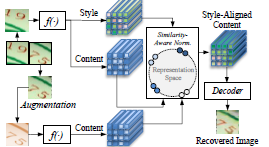
\includegraphics[width=\textwidth]{figure1b.png}
        \caption{Generative representation learning (ours)}
        \label{fig:tiger}
    \end{subfigure}
   
    \caption{Scene text representation learning in (a) the contrastive and (b) the generative manner (ours). We estimate the similarity of the content representations between the augmented patch and its neighboring patch, and align the corresponding styles to reconstruct the augmented patch. Only high-quality representations are distinguishable so that a precise reconstruction can be achieved.}
    \label{fig:f1}
\end{figure}


\begin{figure}
    \centering
    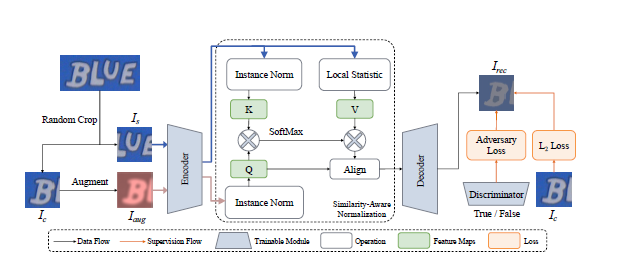
\includegraphics{image1.png}
    \caption{Overview of the proposed generative representation learning scheme. We decouple content and style as two different inputs and guide the network to recover the augmented image. The proposed SimAN module learns to align corresponding styles for different patterns according to the distinguishable representations.}
    \label{fig:my_label}
\end{figure}


\begin{figure}
    \centering
    \begin{subfigure}[b]{0.3\textwidth}
        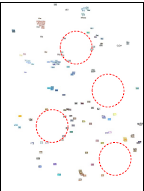
\includegraphics[width=\textwidth]{image5.png}
       \label{fig:gull}
    \end{subfigure}
    
    \begin{subfigure}[b]{0.3\textwidth}
        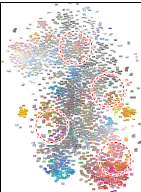
\includegraphics[width=\textwidth]{image.png}
        \label{fig:tiger}
    \end{subfigure}
   
    \caption{Distribution of scene text images containing the word
“the” via t-SNE.We show two distributions of (a) 200 real labeled
samples and (b) 200 real samples and our 2000 synthetic samples.
The large empty space of original distribution might suggest the
lack of diversity of labeled data. After adding our synthetic samples,
the distribution is more even and dense. Best viewed in color.}
    \label{fig:f1}
\end{figure}







\begin{tabular}{c c c c}

    \hline
    Method &Supervision& FID ↓ &Acc. ↑\\
      \\
     \hline
     EditText [57]& ✓ &40.5 &14.9\\
Ours &× &67.9 &57.6\\
\hline
    
\end{tabular}

\printbibliography
\end{document}
